\newpage
\section{Struktura}
    \subsection{Architektura}
    \subsubsection{Backend}
    Do stworzenia systemu, została wykorzystana architektura oparta na usługach chmurowych. Jest to podyktowane dostępnością wszelakich gotowych usług które można w łatwy sposób zintegrować z tworzonymi systemami. W ten sposób nie trzeba tworzyć całej infrastruktury od zera. W celu realizacji pracy wybrana został Firebase, czyli zestaw usług backendowych oferowany przez Google \cite{Firebase}. \\
    Usługi wykorzystywane w ramach tworzenia systemu to Cloud Functions, Authorization i Firestore. \\
    Pierwszą z wykorzystywanych usług jest \textbf{Firestore Database}. Jest to nierelacyjna baza danych, która przechowuje swoje dane w formacie json. W tym komponencie przechowywane są przede wszystkim informacje dotyczące atrakcji turystycznych, w tym:
    \begin{itemize}
        \item nazwa atrakcji,
        \item adres atrakcji,
        \item opis atrakcji,
        \item godziny otwarcia,
        \item ceny biletów,
        \item udogodnienia dla osób niepełnosprawnych,
        \item linki do zdjęć atrakcji
    \end{itemize}
    W bazie danych zamodelowane są również dane dotyczące miast w któych atrakcje mogą się znajdować, używanych języków, walut obsługiwanych przez dane państwa i numerów alarmowych w krajach.
    % Do opisania wszystkie wykorzystywane usługi, co robią, po co są itd.

    \subsubsection{Frontend}
    Aplikacja mobilna, została napisana przy użyciu języka TypeScript \cite{TypeScript} stworzonego przez Microsoft. Jest on nadzbiorem języka JavaScript. Jako statycznie typowany język, pozwala on na lepszą kontrolę typów przez programistów. Jest on także natywnie wspierany przez przeglądarki dzięki transpilacji do JavaScript jednocześnie oferując składnię rozszerzoną o między innymi klasy, enumeratory lub interfejsy. \\
    Do stworzenia samej aplikacji, wykorzystany został framework React Native \cite{ReactNative} który został stworzony przez Meta i wzorowany na popularnej bibliotece React. Pozwala on na tworzenie aplikacji natywnych na platformy mobilne Android oraz iOS przy użyciu JavaScriptu i mechanizmów znanych z biblioteki React. \\
    Wątki kodu wykonywanego w JavaScript komunikują się przy pomocy mostu (\textit{ang. bridge}) z wątkami działającymi natywnie na danej platformie poprzez serializację i deserializację wiadomości wysyłanych z obu rodzajów wątków. \cite{ReactNativeMedium} \cite{ReactNativeNetguru}.
    Dzięki temu rozwiązaniu, można w bardzo łatwy sposób stworzyć kod aplikacji na platformy mobilne, który nie będzie wymagał tworzenia osobnych wersji dla różnych systemów operacyjnych lub tłumaczenia kodu na język używany w innych platformach. \\
    Schemat działania React Native został przedstawiony na rysunku 3.2. \\

    Aplikacja webowa stworzona została przy użyciu języka JavaScript i biblioteki React w wersji 18, dzięki której możliwe jest tworzenie interaktywnych stron internetowych.

    \subsubsection{Baza danych}
    W projekcie został także wykorzystany serwis umożliwiający przechowywanie niestrukturyzowanych danych Cloud Storage od Google \cite{CloudStorage}, w której przechowywane są grafiki. Linki do nich są umieszczone w dokumentowej bazie danych Firestore, które następnie są pobierane przez aplikację napisaną w React Native i wyświetlane użytkownikowi. W bezpłatnej wersji oferowana jest opcja przechowywania 5GB danych co na wystarczyło na potrzeby pisania pracy dyplomowej. \\

    Całą architekturę przedstawia poniższy diagram:
    
    \begin{figure}[H]
        \centering
        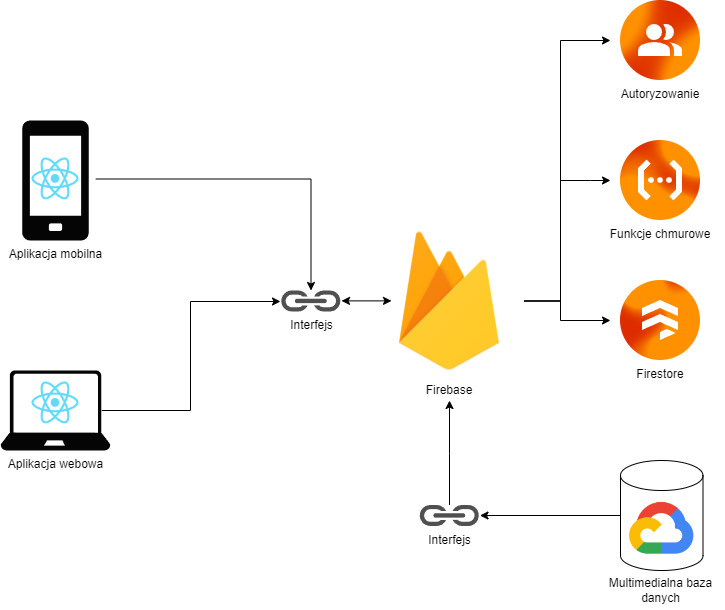
\includegraphics[width=\textwidth]{img/3/architektura.png}
        \caption{Schemat architektury systemu}
        \label{fig:architektura}
    \end{figure}

    \subsection{Stos technologiczny}
    Do wykonania projektu aplikacji, zostały wykorzystane następujące technologie:
    \begin{itemize}
        \item JavaScript,
        \item React,
        \item React Native,
        \item React Navigation,
        \item Expo,
        \item Firestore Database,
        \item Firebase Cloud Functions,
        \item Firebase Authentication,
        \item Google Storage,
    \end{itemize}

    \subsection{Środowisko programistyczne}
    Poszczególne warstwy aplikacji zostały stworzone przy użyciu zintegrowanego środowiska programistycznego (IDE). Mój wybór padł na WebStorm \cite{WebStorm}, gdyż jest on przystosowany do pracy z aplikacjami webowymi, oferuje integrację z systemem kontroli wersji i daje możliwość rozszerzenia edytora za pomocą pluginów. Środowisko to zostało stworzone na bazie IntelliJ IDEA udostępnianego przez JetBrains. \\
    
    Do pracy nad bazą danych, została użyta usługa Firestore Database \cite{Firestore}. Jest to dokumentowa baza danych w której wszystkie dane przechowywane są w formacie json. Jest to naturalny sposób przechowywania obiektów w JavaScript co pozwala na uproszczone przetwarzanie danych przez aplikację. Sam dokumentowy model danych jest prosty w użyciu jednak wymaga innego podejścia do organizacji danych. \\
    
    Użyte zostało także środowisko Android Studio \cite{AndroidStudio}. Jest to oficjalne narzędzie do tworzenia aplikacji mobilnych które zostało stworzone na bazie wcześniej wspomnianego IntelliJ IDEA. Pozwoliło mi to na skonfigurowanie wirtualnego urządzenia z wybraną wersją systemu Android (wersja 12) które następnie było przeze mnie wykorzystywane do testowania działania aplikacji. Android Studio jest dostępne bezpłatnie dla deweloperów i jest sugerowany przez Google jako domyślne rozwiązanie do tworzenia aplikacji mobilnych.

    \begin{figure}[H]
        \centering
        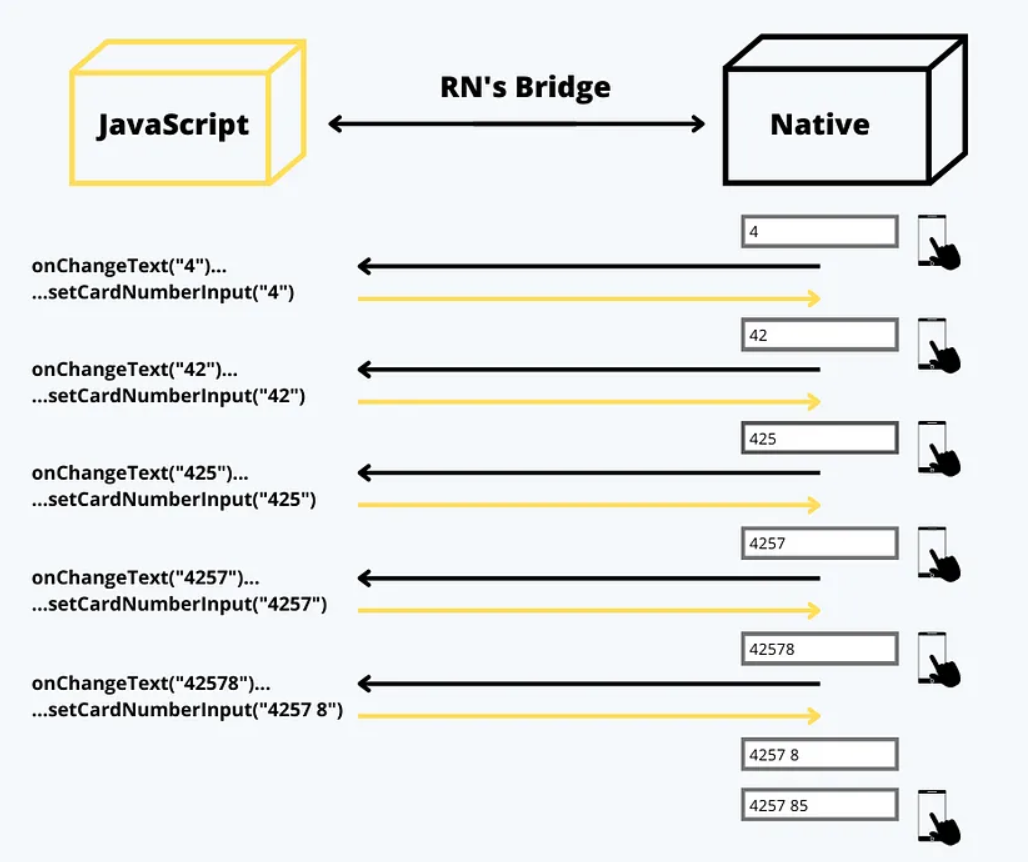
\includegraphics[width=0.8\textwidth]{img/3/react_native_concept.png}
        \caption{Sposób działania mostu w React Native, źródło: \textit{Jakub Kosmal, How does React Native work? Understanding the architecture}}
        \label{fig:react-native}
    \end{figure}